\documentclass{article}

% if you need to pass options to natbib, use, e.g.:
% \PassOptionsToPackage{numbers, compress}{natbib}
% before loading nips_2017
%
% to avoid loading the natbib package, add option nonatbib:
% \usepackage[nonatbib]{nips_2017}

\usepackage[final]{nips_2017}

% to compile a camera-ready version, add the [final] option, e.g.:
% \usepackage[final]{nips_2017}

\usepackage[utf8]{inputenc} % allow utf-8 input
\usepackage[T1]{fontenc}    % use 8-bit T1 fonts
\usepackage{hyperref}       % hyperlinks
\usepackage{url}            % simple URL typesetting
\usepackage{booktabs}       % professional-quality tables
\usepackage{amsfonts}       % blackboard math symbols
\usepackage{nicefrac}       % compact symbols for 1/2, etc.
\usepackage{microtype}      % microtypography
\usepackage{cite}
\usepackage{amsmath}
\usepackage{graphicx} 

\usepackage{algorithm}  
\usepackage{algpseudocode}  
\usepackage{amsmath}  
\renewcommand{\algorithmicrequire}{\textbf{Input:}}  % Use Input in the format of Algorithm  
\renewcommand{\algorithmicensure}{\textbf{Output:}} % Use Output in the format of Algorithm  

\hypersetup{colorlinks,linkcolor={blue},citecolor={blue},urlcolor={blue}}  

\title{CS150A Database \\Course Project}

% The \author macro works with any number of authors. There are two
% commands used to separate the names and addresses of multiple
% authors: \And and \AND.
%
% Using \And between authors leaves it to LaTeX to determine where to
% break the lines. Using \AND forces a line break at that point. So,
% if LaTeX puts 3 of 4 authors names on the first line, and the last
% on the second line, try using \AND instead of \And before the third
% author name.

\author{
  Haoyuan Tian\\
  ID: 2020533013\\
  \texttt{tianhy@shanghaitech.edu.cn} \\
  %% examples of more authors
   \And
  Weiliang Sun\\
  ID: 2020533010\\
  \texttt{sunwl1@shanghaitech.edu.cn}
}

\begin{document}
% \nipsfinalcopy is no longer used

\maketitle

\begin{abstract}

  Compared with developing a novel machine learning algorihtm, building a machine learning system is less theoretical but more engineering, so it is important to get your hands dirty. To build an entire machine learning system, you have to go through some essential steps. We have listed 5 steps which we hope you to go through. Read the instructions of each section before you fill in. You are free to add more sections. \\
  If you use PySpark to implement the algorithms and want to earn some additional points, you should also report your implementation briefly in the last section.
\end{abstract}

\section{Explore the dataset}
\textbf{Our exploration on the dataset:}\\
In this project, we are given an exactly huge dataset, which contains 232744 rows and 19 columns. To avoid
the data which has been discussed in the project explanation pdf, we only focus on those which aren't discussed and also important.\\
So in this part, we mainly explore the data on seven parts of the data as follows: \\
1. Correct Step Duration(sec)
2. Error Step Duration(sec)
3. Correct First Attempt
4. Problem view
5. Corrects
6. Incorrects
7. Hints \\
You can find the detailed implementation of the code in the data visual.ipynb where we explore the data. \\
\textbf{1. Correct Step Duration(sec)}\\
With the help of describe() function, we can get the basic information of the data. \\
\begin{tabular}{|c|c|c|c|c|c|c|c|c|c|}
  \hline
  column name                & count     & mean      & std       & min  & max     & 25\% & 50\% & 75\%  & data type \\
  \hline
  Correct Step Duration(sec) & 181599.00 & 17.924024 & 35.179534 & 0.00 & 1067.00 & 5.00 & 8.00 & 17.00 & float64   \\
  \hline
\end{tabular}

\textbf{Visualization of Correct Step Duration(sec):} Look at figure 1\\
\begin{figure}[htbp]
  \begin{minipage}[c]{3cm}
    \centering
    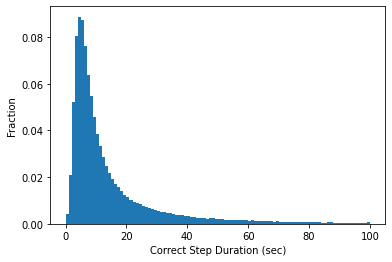
\includegraphics[width=3cm]{correct_step_duration.png}
    \caption{Correct Step Duration(sec)}
  \end{minipage}
  \begin{minipage}[c]{3cm}
    \centering
    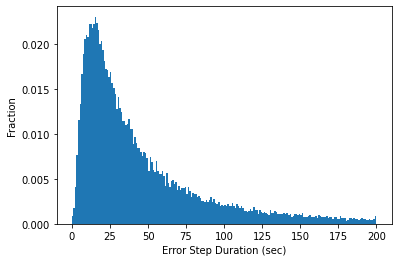
\includegraphics[width=3.cm]{error_step_duration.png}
    \caption{Error Step Duration(sec)}
  \end{minipage}
  \begin{minipage}[c]{3cm}
    \centering
    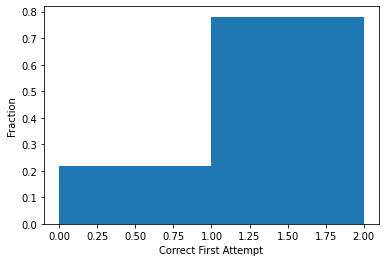
\includegraphics[width=3cm]{correct_first_attempt.png}
    \caption{Correct First Attempt}
  \end{minipage}
  \begin{minipage}[c]{3cm}
    \centering
    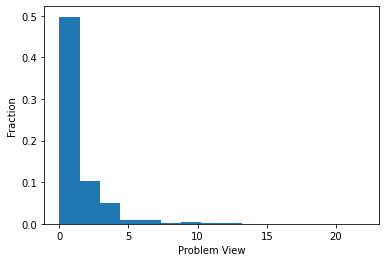
\includegraphics[width=3cm]{problem_view.png}
    \caption{Problem View}
  \end{minipage}
  \begin{minipage}[c]{3cm}
    \centering
    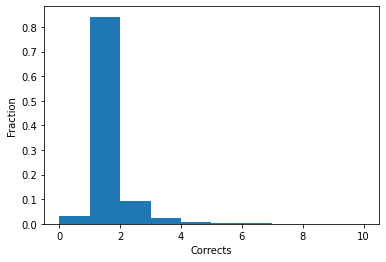
\includegraphics[width=3cm]{corrects.png}
    \caption{Corrects}
  \end{minipage}
  \begin{minipage}[c]{3cm}
    \centering
    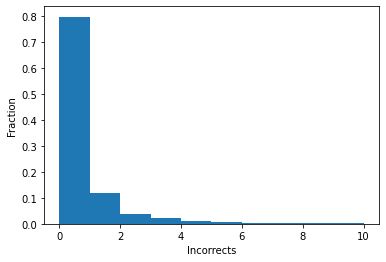
\includegraphics[width=3cm]{incorrects.png}
    \caption{Incorrects}
  \end{minipage}
  \begin{minipage}[c]{3cm}
    \centering
    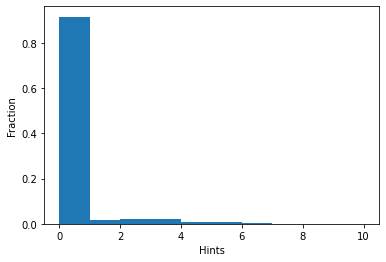
\includegraphics[width=3cm]{hints.png}
    \caption{Hints}
  \end{minipage}
\end{figure}

\textbf{2. Error Step Duration(sec)}\\
\begin{tabular}{|c|c|c|c|c|c|c|c|c|c|}
  \hline
  column name              & count    & mean      & std       & min  & max     & 25\%  & 50\%  & 75\%  & data type \\
  \hline
  Error Step Duration(sec) & 50853.00 & 60.547204 & 89.287960 & 0.00 & 1888.00 & 16.00 & 32.00 & 67.00 & float64   \\
  \hline
\end{tabular}

\textbf{Visualization of Error Step Duration(sec):} Look at figure 2\\
\textbf{3. Correct First Attempt}\\
\begin{tabular}{|c|c|c|c|c|c|c|c|c|c|}
  \hline
  column name           & count     & mean     & std      & min  & max  & 25\% & 50\% & 75\% & data type \\
  \hline
  Correct First Attempt & 232744.00 & 0.780935 & 0.413613 & 0.00 & 1.00 & 1.00 & 1.00 & 1.00 & float64   \\
  \hline
\end{tabular}

\textbf{Visualization of Correct First Attempt:} Look at figure 3\\
\textbf{4. Problem view}\\
\begin{tabular}{|c|c|c|c|c|c|c|c|c|c|}
  \hline
  column name  & count     & mean     & std      & min  & max   & 25\% & 50\% & 75\% & data type \\
  \hline
  Problem View & 232744.00 & 1.602838 & 1.515546 & 1.00 & 21.00 & 1.00 & 1.00 & 2.00 & float64   \\
  \hline
\end{tabular}

\textbf{Visualization of Problem View:} Look at figure 4\\
\textbf{5. Corrects} \\
\begin{tabular}{|c|c|c|c|c|c|c|c|c|c|}
  \hline
  column name & count     & mean     & std      & min  & max   & 25\% & 50\% & 75\% & data type \\
  \hline
  Corrects    & 232744.00 & 1.172636 & 0.797579 & 0.00 & 73.00 & 1.00 & 1.00 & 1.00 & float64   \\
  \hline
\end{tabular}

\textbf{Visualization of Corrects:} Look at figure 5\\
\textbf{6. Incorrects} \\
\begin{tabular}{|c|c|c|c|c|c|c|c|c|c|}
  \hline
  column name & count     & mean     & std      & min  & max    & 25\% & 50\% & 75\% & data type \\
  \hline
  Incorrects  & 232744.00 & 0.475217 & 1.932919 & 0.00 & 175.00 & 0.00 & 0.00 & 0.00 & float64   \\
  \hline
\end{tabular}

\textbf{Visualization of Incorrects:} Look at figure 6\\
\textbf{7. Hints} \\
\begin{tabular}{|c|c|c|c|c|c|c|c|c|c|}
  \hline
  column name & count     & mean     & std      & min  & max   & 25\% & 50\% & 75\% & data type \\
  \hline
  Hints       & 232744.00 & 0.259985 & 1.114299 & 0.00 & 74.00 & 0.00 & 0.00 & 0.00 & float64   \\
  \hline
\end{tabular}

\textbf{Visualization of Hints:} Look at figure 7\\
\section{Data cleaning}
\textcolor{cyan}{Instruction: \\
  Some people treat data cleaning as a part of feature engineering, however we separate them here to make your work clearer. In this section, you should mainly deal with the missing values and the outliers. You can also do some data normalization here.}\\\\
\textbf{Our data cleaning implementation:}\\
\textbf{1. Check if there exists duplicated data:} \\
We use the duplicated() function to check if there exists duplicated data. And we print the sum of
the duplicated data in train and test data, which can be found in data cleaning python file. \\
We found the sum of duplicated data is 0, which means there doesn't exist any duplicated data in the train and test data file.\\
\textbf{2. Check if there exists missing data:} \\
In this part we will check if there exists NaN value in the train and test data. If something strange happens,
we will try to fix the missing data problem in our data file. \\
By using the isnull() function, we can check if there exists NaN value in the train and test data. \\
In our result which is interpreted in the data cleaning python file, we find that columns like Anon Student Id, Problem Hierarchy, Problem Name, Problem View, and Step Name have 0 missing data,
which means in the columns which are important, there doesn't exist any missing data. However, we find some NaN value in the columns
like Step Start Time, Correct Transaction Time, Opportunity and so on. \\
Of course, these missing data has no effect on our prediction, because they make sense at all. For example,
if a student doesn't answer a question, there is no correct transaction time. And those who succeed in the first
attempt will of course get a NaN value in the Opportunity column and Error Step Duration. \\
\textbf{3. Check if the important columns are unique:} \\
In this part, we will check if the important columns are unique by using the duplicated() function. \\
In our result which is interpreted in the data cleaning python file, we find that columns which are primary keys
like Anon Student Id, Problem Hierarchy, Problem Name, Problem View, and Step Name are unique exactly. \\
\textbf{4. Check if there exists some outrange data:} \\
In this part, we will check if there exists some abnormal data, which in our definition calls its outrange.
We set a reasonable range as 500 as the checking range for the abnormal data, and find each column if there exists data out of this range.\\
You can see our implementation in data cleaning python file and it is reported that there is no error, meaning that all data
in some extent are normal enough to support our further exploration.
\section{Feature engineering}
\textcolor{cyan}{Instruction: \\
  In this section, you should select a subset of features and transform them into a data matrix which can be feed into the learning model you choose. Report your work with reasons.}\\\\
\textbf{Your work below:}\\
Works are done in the file feature\_engineering.py. The major work is to convert the original data set to a machine-readable status, including encoding strings to numbers that can be evaluated. Besides, some no use columns should be removed, and we also add some useful columns.\\
\textbf{Aadjusting columns.}
The first step is to drop several useless columns that could disturb the training, or not be in the testing data set as well, such as 'Row', 'Step Start time', 'First Transaction Time', and 'Incorrects', 'Hints', 'Corrects' etc. \\
\textbf{Encoding.}
Before encoding, we divide the 'Problem Hierarchy' column in to 'Problem Unit' and 'Problem Section' to get more details.
We should remember that the computer is better to deal with numbers than strings, intuitively, when the strings should be distinct, the numbers should also be just distinct. We implement a naive encoding to several columns such as 'Anon Student Id', 'Problem Name',
'Problem Unit', 'Problem Section',
'Step Name'.
The key is to always distribute a distinct integer number to a distinct string, and conversely distribute the same integer number to a string that has appeared.\\
\textbf{Dealing with complexes.}
There are special items in the data set, which contains '~~'. We should try to convert it to an machine- understandable words, again numbers. The first is 'Opportunity(Default)', we replace it with an average of all opportunities. As for 'KC(Default)', we replace it with a KC count roughly.\\
The above operations exactly encode such columns, but the performance should not be worth expecting, we should add some new features, considering columns that is near 'Correct First Attempt'.\\
\textbf{New features.} 7 new features we have added is Personal Correct First Attempt Count, Personal Correct First Attempt Rate, and Correct First Attempt Rate per Problem, Correct First Attempt Rate per unit, Correct First Attempt Rate per section, Correct First Attempt Rate per step, and also  Correct First Attempt Rate per KC. Count is like an accumulator and Rate is like an average, both are naive work after we find the exact column, and use udf of pyspark to operate them.\\
The final header of the data set is like 'Anon Student Id,	Problem Name,	Problem View,	Step Name,	Correct First Attempt,	Problem Unit,	Problem Section,	Opportunity Average,	KC Count,	Personal CFAC,	Personal CFAR,	Problem CFAR,	Unit CFAR,	Section CFAR,	Step CFAR,	KC CFAR'.
\textbf{Export.}
The work of this part is exported to './data/train\_pyspark.csv' and './data/test\_pyspark.csv'.

\section{Learning algorithm}
\textcolor{cyan}{Instruction: \\
  In this section, you should describe the learning algorithm you choose and state the reasons why you choose it.}\\\\
\textbf{Your work below:}\\
Algorithm we use and their performances (RMSE) are as follow.\\
MLPRegressor : 0.388670\\
decision tree : 0.514066\\
RandomForest : 0.365582\\
Adaboost : 0.391298\\
XGBoost : 0.419137\\
lightgbm : 0.406405\\
Gradient Decision Tree : 0.420924\\
Logistic Regression : 0.434959\\
Dummy Regression : 0.392797\\
KNN : 0.413511\\
tree bagging : 0.367498\\
knn bagging : 0.402778\\
Dummy bagging : 0.392794\\
We would like to choose algorithms as much as possible so as not to loss any possible best algorithm for training this data set. So our model includes Neural Network and
traditional methods, parametric methods, non-parametric methods, individual models and ensemble learning models.\\
After several trials, we can easily tell that RandomForest and tree bagging are obviously better than others, and we can hardly tell which of them is better than the other.
\section{Hyperparameter selection and model performance}
\textcolor{cyan}{Instruction: \\
  In this section, you should describe the way you choose the hyperparameters of your model, also compare the performance of the model with your chosen hyperparamters with models with sub-optimal hyperparameters}\\\\
\textbf{Your work below:}\\
Since the performance of RandomForest and tree bagging are outstanding, plus the inefficiency of tree bagging, we choose to optimize RandomForest.\\
We use GridSearchCV to try a range of parameters that applied to RandomForestRegressor. Such as for n\_estimators we try a range of range(10, 210, 10) and get the best parameter being 170 (literally we have tried several ranges like (160,210,5), (170,220,5), the bbest retrun is 205 and 215, plus we also try with 190, we can say that the performance from 170 to 220 would not make large difference); for max\_depth we take range(5, 21) and get the best parameter 15, on the base of n\_estimator=170; for max\_leaf\_nodes we take range(100, 1000, 100) and get the best is 900, also on the base of previous optimizations.\\
The the final hyperparameter we choose for a RandomForestRegressor is n\_estimators=170, max\_depth=15, max\_leaf\_nodes=900. It could be better to go more detailed, but running the randomforest is for tons of time is costly so we just stop there. The optimized RandomForestRegressor's RMSE is 0.353911, which is much better then the origin 0.365582.

\section{PySpark implementation (optional)}
We use PySpark to operate the data set when doing feature engineering (feature\_engineering.py). Since the size of the data set is so large that PySpark would help it performan much better than naively
traverse all the time, thanks to distributed processing.\\
The major part of utilizing pyspark is the pyspark.sql.functions. We apply user define functions (udf) all the time to operate the data set by column. It is intuitive to implement a function on a specific column, as well as convert it into udf, then apply the udf to the data set with a specific column. Besides, initialization and some querry operations such as group by, count, distinct are also from pyspark.
\end{document}
